\documentclass[conference]{IEEEtran}
\IEEEoverridecommandlockouts
\usepackage{cite}
\usepackage{amsmath}
\usepackage{newtxtext,newtxmath}
\usepackage{graphicx}
\usepackage{booktabs}
\usepackage{tikz}
\usetikzlibrary{arrows.meta,positioning,calc}
\usepackage{url}
\usepackage[hidelinks]{hyperref}
\hypersetup{
  pdftitle={Do Smart Grid Intrusion Detectors Learn Attacks or Operating Conditions? Evidence from a PMU-Relay Testbed and an IEEE 14-Bus Simulation},
  pdfauthor={Haider Md. Faiyaz Hussain Shahi},
  pdfkeywords={smart grid, intrusion detection, phasor measurement unit, false data injection, state estimation, machine learning}
}

\begin{document}

\title{Do Smart Grid Intrusion Detectors Learn Attacks or Operating Conditions? Evidence from a PMU-Relay Testbed and an IEEE 14-Bus Simulation}

\author{\IEEEauthorblockN{Haider Md. Faiyaz Hussain Shahi}
\IEEEauthorblockA{\textit{Independent Researcher} \\
\url{https://orcid.org/0009-0004-0940-9096} \\
shahihussainofficial1@gmail.com \\
DOI: \href{https://doi.org/10.5281/zenodo.24054176}{10.5281/zenodo.24054176}}
}

\maketitle

\begin{abstract}
Machine learning detectors of cyber attacks on power systems are often evaluated with a random split of samples. We study whether such detectors learn attacks or operating conditions, using a public dataset recorded on a PMU-relay testbed and a 42-day simulation of the IEEE 14-bus system with phasor measurement units and false data injection (FDI). On the testbed data, a random forest separates attacks from natural events with a macro-F1 of 0.90 under a random split but only 0.61 when whole sets of operating conditions are held out, with an accuracy below the majority-class baseline; the sets themselves can be identified with 95.5\% accuracy from normal-operation samples. Load-independent physics features, including sequence-component ratios and consistency between the two ends of a line, reduce the gap between the protocols from 0.29 to 0.04 but do not raise the grouped score above 0.63. In the simulation, stealthy FDI constructed to preserve the state-estimation residual bypasses the chi-square bad data detector (1.1\% detection). A random forest on PMU measurements and the residual detects 99.9\% of stealthy attacks on future days and 86\% of attacks on buses not seen during training, at false-alarm rates of 1.4--1.8\%, provided that its alarm threshold is calibrated on held-out normal data; with the default threshold it detects 62\% despite a ROC-AUC of 0.996. We release the simulation and evaluation code.
\end{abstract}

\begin{IEEEkeywords}
smart grid, intrusion detection, phasor measurement unit, false data injection, state estimation, machine learning
\end{IEEEkeywords}

\section{Introduction}
Protection and monitoring in modern transmission grids rely on networked intelligent electronic devices (IEDs) and phasor measurement units (PMUs), which stream time-synchronized voltage and current phasors to a phasor data concentrator (PDC) and the control room~\cite{phadke2008pmu,ieee2011c37118}. The same communication network exposes the grid to cyber attacks: an intruder who reaches the substation network can send trip commands to relays, change relay settings or inject false measurements~\cite{morris2014dataset,liu2011fdi}. Machine learning classifiers that separate attacks from natural faults and normal operation have therefore been proposed for both PMU-relay data~\cite{hink2014ml,pan2015hybrid,pan2015classification} and state-estimation data~\cite{ozay2016ml,esmalifalak2017stealthy,he2017deep}.

For a detector to be useful it must work under operating conditions that were not seen during training. Machine learning for security is known to be vulnerable to evaluation pitfalls such as data snooping and spurious correlations~\cite{sommer2010closed,arp2022dos,engelen2021cicids}, and leakage between training and test data is a recurrent cause of irreproducible results~\cite{kaufman2012leakage,kapoor2023leakage}. In power systems, samples recorded under the same load level and fault scenario are strongly correlated, so a random split of samples places near-identical operating points in both training and test data.

This paper examines this issue with two complementary data sources: the public power system attack dataset recorded on a PMU-relay testbed at Mississippi State University and Oak Ridge National Laboratory~\cite{morris2014dataset}, and a time-series simulation of the IEEE 14-bus system with PMUs, weighted least-squares (WLS) state estimation and false data injection (FDI). The contributions are:
\begin{enumerate}
\item On the testbed data, we show that a random split of samples rewards recognition of the operating condition: the 15 sets of the dataset can be told apart with 95.5\% accuracy from normal-operation samples alone, and attack detection drops close to the majority-class level when whole sets are held out.
\item We evaluate load-independent physics features (sequence-component ratios, phase unbalance and line-end consistency) and unlabeled per-set normalization, and quantify how much they reduce the gap between the two protocols.
\item In the simulation, where the ground truth of every sample is known, we compare the chi-square bad data detector (BDD) with four lightweight classifiers under random, chronological and unseen-target splits, and show which feature and model choices generalize to attacks on buses not seen during training.
\end{enumerate}

\section{Related Work}
Hink \emph{et al.}~\cite{hink2014ml} applied several machine learning classifiers to the testbed data, and Pan \emph{et al.} combined synchrophasor measurements and logs in a data-mining-based hybrid intrusion detection system~\cite{pan2015hybrid} and in a classifier of disturbances and attacks~\cite{pan2015classification}. Liu \emph{et al.}~\cite{liu2011fdi} showed that an attacker who knows the measurement model can inject false data $a=Hc$ that leaves the WLS residual unchanged and therefore bypasses the BDD. Ozay \emph{et al.}~\cite{ozay2016ml}, Esmalifalak \emph{et al.}~\cite{esmalifalak2017stealthy} and He \emph{et al.}~\cite{he2017deep} detected such attacks with machine learning methods, including deep learning in~\cite{he2017deep}, on simulated IEEE test systems. General pitfalls of machine learning for intrusion detection are discussed in~\cite{sommer2010closed,arp2022dos}, and labeling and design problems of a widely used network intrusion dataset are documented in~\cite{engelen2021cicids}. We apply such scrutiny to power system attack detection, together with a simulation in which operating conditions and attack targets are controlled.

\section{Systems and Data}
\subsection{PMU-Relay Testbed}
Fig.~\ref{fig:testbed} shows the testbed, redrawn from the dataset documentation~\cite{morris2014dataset}. Two generators G1 and G2 feed a load bus B2 through lines L1 and L2. Each line end has a breaker (BR1--BR4) controlled by an IED with an integrated PMU (R1--R4) that uses distance protection. The IEDs communicate through a substation switch with a PDC and the control room, which hosts a control panel, Snort, a syslog server and OpenPDC. The 37 scenarios comprise single-line-to-ground faults and line maintenance (8 natural events), normal operation with load changes (1) and 28 attacks: data injection that imitates a fault, remote tripping command injection and relay setting changes. Each sample contains 116 PMU measurements (29 per relay: phase and sequence voltage and current phasors, frequency, rate of change of frequency, apparent impedance and a status flag) and 12 control-panel, relay and Snort log columns. The released data consist of 15 sets, each a 1\% random sample of the 37 scenarios, with 78{,}377 samples in total; 71.0\% of the samples belong to attack scenarios. Only the scenario number is available for each sample; time stamps are not released.

\begin{figure}[t]
\centering
\resizebox{\columnwidth}{!}{% Single-line and communication diagram of the MSU/ORNL power system testbed
% (redrawn from the dataset documentation).
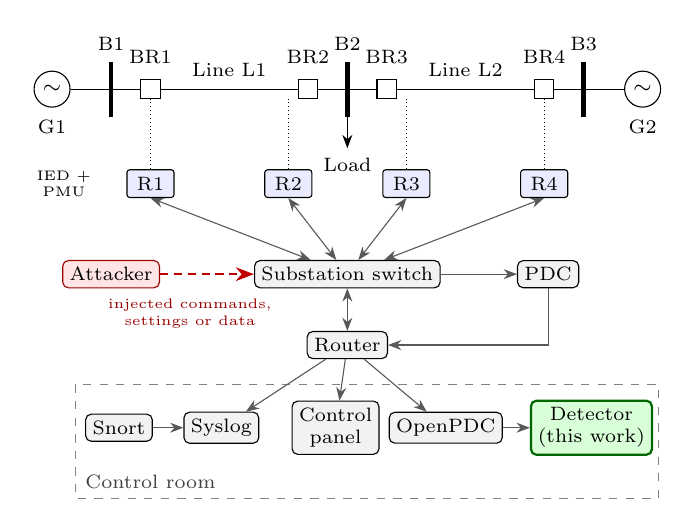
\begin{tikzpicture}[
  font=\footnotesize, >=Stealth,
  bus/.style={line width=1.6pt},
  brk/.style={draw, fill=white, minimum width=7pt, minimum height=7pt, inner sep=0pt},
  ied/.style={draw, rounded corners=1pt, fill=blue!8, minimum width=17pt, minimum height=10pt, inner sep=1pt, font=\scriptsize},
  box/.style={draw, rounded corners=2pt, fill=gray!10, align=center, inner sep=2.5pt, font=\scriptsize},
  comm/.style={->, thin, gray!70!black},
  atk/.style={->, thick, red!75!black, densely dashed}
]
% generators and buses
\node[draw, circle, minimum size=13pt, inner sep=0pt] (g1) at (0,0) {$\sim$};
\node[below=1pt of g1, font=\scriptsize] {G1};
\draw[bus] (0.75,-0.35) -- (0.75,0.35) node[above, font=\scriptsize] {B1};
\draw (g1) -- (0.75,0);
\node[draw, circle, minimum size=13pt, inner sep=0pt] (g2) at (7.5,0) {$\sim$};
\node[below=1pt of g2, font=\scriptsize] {G2};
\draw[bus] (6.75,-0.35) -- (6.75,0.35) node[above, font=\scriptsize] {B3};
\draw (g2) -- (6.75,0);
\draw[bus] (3.75,-0.35) -- (3.75,0.35) node[above, font=\scriptsize] {B2};
\draw[->] (3.75,-0.35) -- (3.75,-0.75) node[below, font=\scriptsize] {Load};
% breakers and lines
\node[brk] (br1) at (1.25,0) {}; \node[above=2pt of br1, font=\scriptsize] {BR1};
\node[brk] (br2) at (3.25,0) {}; \node[above=2pt of br2, font=\scriptsize] {BR2};
\node[brk] (br3) at (4.25,0) {}; \node[above=2pt of br3, font=\scriptsize] {BR3};
\node[brk] (br4) at (6.25,0) {}; \node[above=2pt of br4, font=\scriptsize] {BR4};
\draw (0.75,0) -- (br1) -- node[above=1pt, font=\scriptsize] {Line L1} (br2) -- (3.75,0) -- (br3) -- node[above=1pt, font=\scriptsize] {Line L2} (br4) -- (6.75,0);
% relays / PMUs
\foreach \i/\x in {1/1.25,2/3.0,3/4.5,4/6.25}{
  \node[ied] (r\i) at (\x,-1.2) {R\i};
  \draw[densely dotted] (r\i) -- (\x,-0.12);
}
\node[font=\tiny, align=center] at (0.15,-1.2) {IED +\\PMU};
% network
\node[box] (sw) at (3.75,-2.35) {Substation switch};
\foreach \i in {1,...,4}{ \draw[comm, <->] (r\i.south) -- (sw); }
\node[box] (pdc) at (6.3,-2.35) {PDC};
\draw[comm] (sw) -- (pdc);
\node[box] (rt) at (3.75,-3.25) {Router};
\draw[comm, <->] (sw) -- (rt);
\draw[comm] (pdc) |- (rt);
% control room
\node[box] (snort) at (0.85,-4.3) {Snort};
\node[box] (sys) at (2.15,-4.3) {Syslog};
\node[box] (cp) at (3.6,-4.3) {Control\\panel};
\node[box] (opdc) at (5.0,-4.3) {OpenPDC};
\node[box, fill=green!15, draw=green!40!black, thick] (ids) at (6.85,-4.3) {Detector\\(this work)};
\draw[dashed, gray] (0.3,-3.75) rectangle (7.7,-5.2);
\node[font=\scriptsize, gray!50!black, anchor=south west] at (0.3,-5.2) {Control room};
\draw[comm] (rt) -- (sys);
\draw[comm] (rt) -- (cp);
\draw[comm] (rt) -- (opdc);
\draw[comm] (opdc) -- (ids);
\draw[comm] (snort) -- (sys);
% attacker
\node[box, fill=red!10, draw=red!60!black] (att) at (0.75,-2.35) {Attacker};
\draw[atk] (att) -- (sw);
\node[font=\tiny, red!60!black, align=center] at (1.75,-2.85) {injected commands,\\settings or data};
\end{tikzpicture}
}
\caption{Single-line and communication diagram of the PMU-relay testbed (redrawn from~\cite{morris2014dataset}). Each IED (R1--R4) measures the phasors at its breaker and trips it on a detected fault or on command.}
\label{fig:testbed}
\end{figure}

\subsection{IEEE 14-Bus Simulation}
We simulate the IEEE 14-bus system (Fig.~\ref{fig:ieee14}) with pandapower~\cite{thurner2018pandapower} for 42 days at a 2-minute resolution (30{,}240 AC power flows). Bus loads follow a common daily and weekly profile multiplied by bus-specific slow random walks and minute-level noise, and generator set-points follow the total load. PMUs at buses 2, 6, 7 and 9 measure the bus voltage phasor and the current phasors of all incident branches, giving $m=19$ complex measurements for $n=14$ complex states. Because PMU measurements are linear in the complex bus voltages $x$, the model is $z=Hx+e$ with $H$ built from the branch admittances; we verified that $H$ has full column rank. The noise $e$ is complex Gaussian with a standard deviation of 0.5\% of the measurement magnitude, well within the 1\% total vector error of the synchrophasor standard~\cite{ieee2011c37118}. The control room computes the WLS estimate $\hat{x}=(H^{\mathsf H}WH)^{-1}H^{\mathsf H}Wz$ and the residual statistic $J=r^{\mathsf H}Wr$ with $r=z-H\hat{x}$, and the BDD raises an alarm when $J$ exceeds the 99th percentile of a chi-square distribution with $2(m-n)=10$ degrees of freedom.

\begin{figure}[t]
\centering
\resizebox{0.72\columnwidth}{!}{% Schematic single-line diagram of the IEEE 14-bus system with PMU placement.
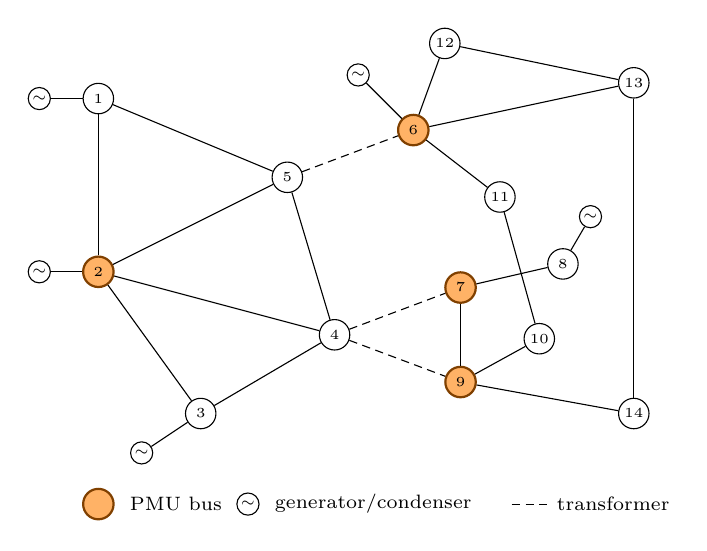
\begin{tikzpicture}[
  font=\scriptsize, >=Stealth,
  bus/.style={draw, circle, fill=white, minimum size=11pt, inner sep=0pt, font=\tiny},
  pmu/.style={bus, fill=orange!60, draw=orange!50!black, thick},
  gen/.style={draw, circle, minimum size=8pt, inner sep=0pt, font=\tiny}
]
\node[bus] (b1)  at (0,4.0) {1};
\node[pmu] (b2)  at (0,1.8) {2};
\node[bus] (b3)  at (1.3,0) {3};
\node[bus] (b4)  at (3.0,1.0) {4};
\node[bus] (b5)  at (2.4,3.0) {5};
\node[pmu] (b6)  at (4.0,3.6) {6};
\node[pmu] (b7)  at (4.6,1.6) {7};
\node[bus] (b8)  at (5.9,1.9) {8};
\node[pmu] (b9)  at (4.6,0.4) {9};
\node[bus] (b10) at (5.6,0.95) {10};
\node[bus] (b11) at (5.1,2.75) {11};
\node[bus] (b12) at (4.4,4.7) {12};
\node[bus] (b13) at (6.8,4.2) {13};
\node[bus] (b14) at (6.8,0.0) {14};
\foreach \a/\b in {1/2,1/5,2/3,2/4,2/5,3/4,4/5,6/11,6/12,6/13,7/8,7/9,9/10,9/14,10/11,12/13,13/14}{
  \draw (b\a) -- (b\b);
}
% transformer branches (dashed)
\foreach \a/\b in {4/7,4/9,5/6}{ \draw[densely dashed] (b\a) -- (b\b); }
% sources
\node[gen] (s1) at (-0.75,4.0) {$\sim$}; \draw (s1) -- (b1);
\node[gen] (s2) at (-0.75,1.8) {$\sim$}; \draw (s2) -- (b2);
\node[gen] (s3) at (0.55,-0.5) {$\sim$}; \draw (s3) -- (b3);
\node[gen] (s6) at (3.3,4.3) {$\sim$}; \draw (s6) -- (b6);
\node[gen] (s8) at (6.25,2.5) {$\sim$}; \draw (s8) -- (b8);
% legend
\node[pmu] (lp) at (0.0,-1.15) {};
\node[right=2pt of lp, font=\scriptsize] {PMU bus};
\node[gen] (lg) at (1.9,-1.15) {$\sim$};
\node[right=2pt of lg, font=\scriptsize] {generator/condenser};
\draw[densely dashed] (5.25,-1.15) -- (5.7,-1.15) node[right, font=\scriptsize] {transformer};
\end{tikzpicture}
}

\vspace{4pt}
\resizebox{\columnwidth}{!}{% Detection pipeline used in the simulation.
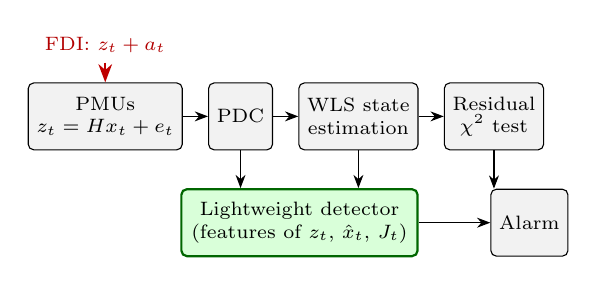
\begin{tikzpicture}[
  font=\scriptsize, >=Stealth, node distance=0.32cm,
  blk/.style={draw, rounded corners=2pt, fill=gray!10, align=center, inner sep=3pt, minimum height=0.85cm},
  new/.style={blk, fill=green!15, draw=green!40!black, thick},
  atk/.style={->, thick, red!75!black, densely dashed}
]
\node[blk] (pmu) {PMUs\\$z_t=Hx_t+e_t$};
\node[blk, right=of pmu] (pdc) {PDC};
\node[blk, right=of pdc] (se) {WLS state\\estimation};
\node[blk, right=of se] (bdd) {Residual\\$\chi^2$ test};
\node[new, minimum width=3.0cm] (ml) at ($(pdc)!0.5!(se) + (0,-1.35)$) {Lightweight detector\\(features of $z_t$, $\hat{x}_t$, $J_t$)};
\node[blk] (al) at ($(bdd |- ml) + (0.45,0)$) {Alarm};
\draw[->] (pmu) -- (pdc);
\draw[->] (pdc) -- (se);
\draw[->] (se) -- (bdd);
\draw[->] (pdc.south) -- (pdc.south |- ml.north);
\draw[->] (se.south) -- (se.south |- ml.north);
\draw[->] (bdd.south) -- (bdd.south |- al.north);
\draw[->] (ml) -- (al);
\node[red!70!black, above=0.25cm of pmu, align=center] (a) {FDI: $z_t+a_t$};
\draw[atk] (a) -- (pmu);
\end{tikzpicture}
}
\caption{Top: IEEE 14-bus system with the four PMU buses. Bottom: simulated measurement and detection chain. The detector runs next to state estimation and uses the PMU data, the state estimate and the residual.}
\label{fig:ieee14}
\end{figure}

About 20\% of the time is under attack, in episodes of 10--60 minutes separated by 30--240 minutes. Each episode is, with equal probability, either a \emph{random FDI}, which scales two to four measurement channels by 5--15\% and rotates them by up to 3$^\circ$, or a \emph{stealthy FDI}, $a=Hc$~\cite{liu2011fdi}, where $c$ changes the voltage of one randomly chosen non-reference bus by 1--5\% in magnitude and 0.5--3$^\circ$ in angle. The simulation contains 175 random and 172 stealthy episodes.

\section{Detection Methods and Protocols}
\subsection{Testbed Features}
Besides the raw PMU columns (\emph{raw}) and the raw columns with the logs (\emph{raw+logs}), we compute 62 \emph{physics} features that do not depend on the load level: for each relay, the ratios of negative- and zero-sequence to positive-sequence current and voltage, the phase current and voltage unbalance, the ratios of the largest phase current and smallest phase voltage to their means, the absolute frequency deviation, the absolute rate of change of frequency, an indicator for an infinite apparent impedance (open breaker) and the status flag; and, for each line, the absolute differences of these unbalance features between its two ends and the log-ratio of the positive-sequence currents at both ends. A natural fault on a line is seen by the relays at both ends, whereas data injected into one relay is not, so these differences are intended to expose imitated faults. As a second approach, \emph{set-normalized} features are the raw PMU columns standardized by the median and interquartile range of all samples of the same set, without labels; this mimics a monitor that normalizes measurements by the recent operating point.

\subsection{Simulation Features}
\emph{Meas.} contains the magnitude and angle of the 19 PMU phasors. \emph{Meas.+residual} adds $J$ and the largest normalized residual. \emph{Temporal} further adds, for every phasor and every estimated state, the deviation from its median over the preceding 60 minutes, computed causally. \emph{Aggregate} is a target-agnostic set of six features: $J$, the largest normalized residual, and the largest deviation from the trailing median over all measurement magnitudes, measurement angles, estimated voltage magnitudes and estimated angles. We also test a training-free \emph{max.-deviation} detector, which raises an alarm when the largest robust z-score of the state deviations exceeds its 99th percentile on normal training samples.

\subsection{Classifiers and Protocols}
We use logistic regression (LR), a decision tree of depth 10 (DT), a random forest with 100 trees (RF)~\cite{breiman2001rf}, all implemented with scikit-learn~\cite{pedregosa2011sklearn}, and gradient-boosted trees with 300 iterations from the LightGBM library (LGBM)~\cite{ke2017lightgbm}, with balanced class weights and fixed hyperparameters. On the testbed data we compare a stratified random 70/30 split with leave-one-set-out (LOSO) cross-validation over the 15 sets, for the binary task (attack versus natural event or normal operation) and for the three-class and 37-scenario tasks. In the simulation we compare a random 70/30 split of samples; a chronological split (days 1--29 for training, 30--42 for testing); and two unseen-target splits, in which stealthy attacks on one half of the buses (even- or odd-numbered) are removed from the training period and only these appear in the test period. We report the macro-F1 score, the detection rate per attack type, the false-alarm rate (FAR) on normal samples, the fraction of attack episodes with at least one alarm, and the ROC-AUC between stealthy-attack and normal test samples.

\section{Results}
\subsection{Testbed: Operating Condition Instead of Attack}
A random forest trained on the raw PMU columns of normal-operation samples identifies the set of held-out normal-operation samples with 95.5\% accuracy, so each set corresponds to a recognizably different operating condition. Fig.~\ref{fig:real} and Table~\ref{tab:real} show the consequence for attack detection. With a random split the RF reaches a binary macro-F1 of 0.90 (accuracy 91.7\%). With LOSO its macro-F1 is 0.61 and its accuracy 68.9\%, below the 71.0\% obtained by always predicting ``attack''; it detects 80\% of attack samples but raises alarms on 59\% of natural-event and normal samples. The per-set LOSO macro-F1 ranges from 0.59 to 0.65, so the drop is not caused by a single unusual set. No feature set or model exceeds a LOSO macro-F1 of 0.63. The log columns add nothing (0.61 with and without them) because the Snort and control-panel logs contain only 2--7 nonzero entries each in 78{,}377 samples. The multiclass tasks collapse in the same way: the three-class macro-F1 of the RF falls from 0.90 to 0.62 and the 37-scenario accuracy from 82.4\% to 20.8\%.

The physics features behave differently from the raw ones. Their random-split macro-F1 is only 0.67, but their LOSO macro-F1 is 0.63, the highest of all; the gap between the protocols shrinks from 0.29 to 0.04. Load-independent features thus remove the shortcut, and their random-split score is an honest estimate, but they do not recover more information. Set normalization raises the random-split score to 0.94 and leaves the LOSO score at 0.61. Linear models show almost no gap (LR: 0.57 versus 0.56) because they cannot memorize operating points, but their scores are close to chance.

\begin{figure}[t]
\centering
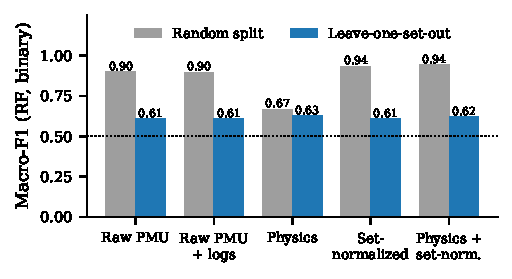
\includegraphics[width=\columnwidth]{figures/real_protocols.pdf}
\caption{Binary macro-F1 of the random forest on the testbed data with a random split and with leave-one-set-out. The dotted line marks 0.5.}
\label{fig:real}
\end{figure}

\begin{table}[t]
\caption{Testbed, binary task: macro-F1 (random split / LOSO) and, for the RF under LOSO, detection rate / false-alarm rate}
\label{tab:real}
\centering
\footnotesize
\setlength{\tabcolsep}{2.3pt}
\begin{tabular}{@{}lccccc@{}}
\toprule
Features & LR & DT & RF & LGBM & RF det./FAR \\
\midrule
Raw PMU & 0.57/0.56 & 0.65/0.58 & 0.90/0.61 & 0.76/0.60 & 0.80/0.59 \\
Raw PMU + logs & 0.58/0.57 & 0.65/0.58 & 0.90/0.61 & 0.76/0.60 & 0.80/0.59 \\
Physics & 0.53/0.52 & 0.53/0.56 & 0.67/0.63 & 0.63/0.60 & 0.82/0.57 \\
Set-normalized & 0.57/0.56 & 0.65/0.57 & 0.94/0.61 & 0.84/0.61 & 0.87/0.67 \\
Physics + set-norm. & 0.57/0.56 & 0.54/0.56 & 0.94/0.62 & 0.84/0.62 & 0.86/0.63 \\
\bottomrule
\end{tabular}
\end{table}

These results suggest that many attack samples in this dataset cannot be distinguished from natural events by their PMU measurements alone. This is consistent with the scenario definitions: a data injection attack imitates a fault, a relay setting change is combined with a real fault, and a command injection opens a breaker as during maintenance. In addition, labels are assigned per scenario, so any samples recorded before an attack takes effect also carry the attack label and describe the scenario rather than the physical state of the sample; without time stamps, we could not determine how many such samples the data contain.

\subsection{Simulation: Stealthy FDI Bypasses the BDD}
Fig.~\ref{fig:ts} shows one test day. Random FDI raises $J$ by two orders of magnitude, whereas stealthy FDI leaves it unchanged. Over the whole simulation the BDD detects 78\% of random-FDI samples (88\% of the episodes) and 1.1\% of stealthy-FDI samples at a false-alarm rate of 1.3\%; the stealthy detection rate is at the level of the false-alarm rate, so the BDD is blind to these attacks, as predicted in~\cite{liu2011fdi}. The 17\% of stealthy episodes that contain at least one BDD alarm are consistent with false alarms that happen to fall within episodes of up to 30 samples.

\begin{figure}[t]
\centering
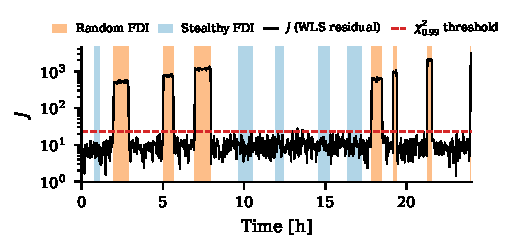
\includegraphics[width=\columnwidth]{figures/sim_timeseries.pdf}
\caption{Residual statistic $J$ and BDD threshold over one test day of the simulation. Shaded intervals mark random (orange) and stealthy (blue) FDI episodes.}
\label{fig:ts}
\end{figure}

\subsection{Simulation: Generalization of Learned Detectors}
With a random split, RF and LGBM detect 100\% of the stealthy samples from the PMU measurements alone. This figure is again optimistic, because samples of the same 10--60-minute episode are present in both training and test data. Table~\ref{tab:sim} and Fig.~\ref{fig:sim} report the chronological and unseen-target splits with calibrated alarm thresholds: each model is refit on days 1--23, and its threshold is set to a 1\% false-alarm rate on the normal samples of days 24--29. On future days, the RF with measurements and residual detects 99.9\% of the stealthy samples at a false-alarm rate of 1.4\%, and LGBM 95.9\% at 0.9\%. When the attacked buses have not been seen during training, the RF detects 86\% of the stealthy samples and 90\% of the episodes at a false-alarm rate of 1.8\%, and LGBM 77\% at 1.3\%; the decision tree drops to 40\%.

The alarm threshold matters as much as the model. With the default probability threshold of 0.5, the RF trained on the full training period detects only 62\% of the unseen-target stealthy samples, although its ROC-AUC on these samples is 0.996. The tree ensembles keep ranking unseen attacks above normal operation (AUC 0.97--1.00 for RF and LGBM on all feature sets except the aggregate one), but their predicted probabilities for attacks on new buses are lower, so a threshold learned from the training labels is too high. Calibrating the threshold on held-out normal data corrects this; the achieved false-alarm rates on the test period (0.1--3.2\%) are close to, but not always below, the 1\% target.

The additional features did not improve generalization. With the temporal features the RF detects only 62\% of the unseen-target attacks, possibly because the per-channel deviations encode the location of the attacks seen in training. The target-agnostic aggregate features reach an AUC of 0.68--0.85 but detect at most 43\% at the calibrated threshold (the decision tree on these features raised no alarm, probably because its few distinct output values place the calibrated threshold at its largest score), and the training-free max.-deviation detector detects 6\% of the stealthy samples. In normal operation, the largest deviation of any estimated bus voltage from its 60-minute median reaches 4.5\% in magnitude and 2.5$^\circ$ in angle (99th percentiles), the same order as the attacks, so a single largest-deviation statistic does not separate them from normal operation.

\begin{figure}[t]
\centering
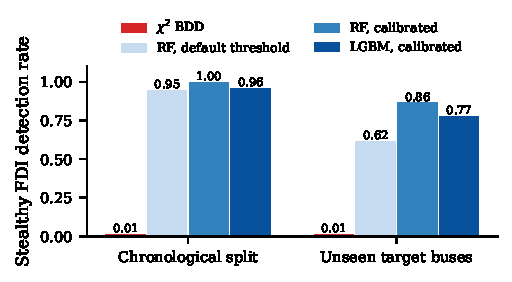
\includegraphics[width=\columnwidth]{figures/sim_detection.pdf}
\caption{Stealthy-FDI detection rate in the simulation for the BDD and for RF and LGBM on measurements and residual, with the default threshold and with a threshold calibrated to 1\% false alarms on held-out normal data (unseen targets: mean of both partitions).}
\label{fig:sim}
\end{figure}

\begin{table}[t]
\caption{Simulation results with calibrated thresholds. Det. R/S: detection rate of random/stealthy FDI samples. Unseen targets: mean of the two partitions.}
\label{tab:sim}
\centering
\footnotesize
\setlength{\tabcolsep}{2.2pt}
\begin{tabular}{@{}llccccccc@{}}
\toprule
 & & \multicolumn{3}{c}{Chronological} & \multicolumn{3}{c}{Unseen targets} \\
\cmidrule(lr){3-5}\cmidrule(lr){6-8}
Features & Model & Det.\,R & Det.\,S & FAR & Det.\,S & FAR & AUC \\
\midrule
\multicolumn{2}{@{}l}{$\chi^2$ BDD} & 0.80 & 0.01 & 0.012 & 0.01 & 0.012 & -- \\
\multicolumn{2}{@{}l}{Max.-deviation} & 0.00 & 0.06 & 0.006 & 0.06 & 0.006 & -- \\
\midrule
Meas. & LR & 0.20 & 0.78 & 0.003 & 0.64 & 0.003 & 0.672 \\
Meas. & DT & 0.23 & 0.79 & 0.009 & 0.44 & 0.016 & 0.715 \\
Meas. & RF & 0.76 & 0.97 & 0.019 & 0.87 & 0.025 & 0.994 \\
Meas. & LGBM & 0.75 & 0.94 & 0.001 & 0.76 & 0.006 & 0.989 \\
\midrule
Meas. + residual & LR & 0.80 & 0.85 & 0.005 & 0.65 & 0.002 & 0.735 \\
Meas. + residual & DT & 0.80 & 0.82 & 0.006 & 0.40 & 0.002 & 0.643 \\
Meas. + residual & RF & 0.88 & 1.00 & 0.014 & 0.86 & 0.018 & 0.996 \\
Meas. + residual & LGBM & 0.90 & 0.96 & 0.009 & 0.77 & 0.013 & 0.975 \\
\midrule
Temporal & LR & 0.80 & 0.80 & 0.007 & 0.68 & 0.008 & 0.794 \\
Temporal & DT & 0.80 & 0.85 & 0.011 & 0.34 & 0.011 & 0.591 \\
Temporal & RF & 0.87 & 0.96 & 0.032 & 0.62 & 0.026 & 0.975 \\
Temporal & LGBM & 0.87 & 0.95 & 0.016 & 0.57 & 0.014 & 0.968 \\
\midrule
Aggregate & LR & 0.80 & 0.45 & 0.009 & 0.43 & 0.006 & 0.836 \\
Aggregate & DT & 0.00 & 0.00 & 0.000 & 0.00 & 0.000 & 0.676 \\
Aggregate & RF & 0.80 & 0.31 & 0.002 & 0.26 & 0.003 & 0.846 \\
Aggregate & LGBM & 0.79 & 0.32 & 0.002 & 0.36 & 0.003 & 0.793 \\
\bottomrule
\end{tabular}
\end{table}

\section{Discussion}
\textbf{Evaluation.} On the testbed data, a random split of samples measures how well a classifier recognizes the operating condition of a set, not how well it detects attacks under new conditions. We recommend grouping the evaluation by set, reporting the majority-class baseline and the false-alarm rate, and comparing random-split and grouped scores; a large gap indicates a shortcut. In PMU-based FDI detection, the same issue appears as leakage between samples of one episode, and the more demanding question is whether attacks on new targets are detected. Reporting a threshold-free measure such as the ROC-AUC alongside detection rates separates the ability to rank attacks from the choice of threshold.

\textbf{Deployment.} The simulation suggests that a tree ensemble on PMU measurements and the WLS residual, with its alarm threshold calibrated on recent normal operation, can complement the BDD against stealthy FDI, including attacks on buses not seen during training. On the testbed data, by contrast, per-sample PMU features were not sufficient in our experiments; detecting imitated faults and malicious commands likely requires sequences of measurements and the context of relay commands and settings. On a laptop CPU, the binary testbed models need 44\,kB and 0.13\,ms per sample (DT) and 1.0\,MB and 1.3\,ms (LGBM), compatible with an embedded gateway or PDC, whereas the RF needs 73\,MB and 31\,ms.

\textbf{Limitations.} The released testbed data contain neither time stamps nor run identifiers, so we could not label samples by their physical state or group them more finely than by set. The simulation uses one test system, a linear PMU measurement model, an attacker who knows $H$, synthetic load profiles and one noise level, and it does not model communication delays or missing data. Hyperparameters were fixed and not tuned.

\section{Conclusion}
On a public PMU-relay testbed dataset, attack detectors appear accurate with a random split of samples but fall to the majority-class level when entire sets of operating conditions are held out, and the sets are recognizable from normal operation alone, which indicates that the classifiers learn the operating condition. Load-independent physics features remove this shortcut but indicate that the per-sample PMU data carry little information about the attacks. In an IEEE 14-bus simulation with exact ground truth, stealthy false data injection bypasses the chi-square detector, while a random forest on PMU measurements and the state-estimation residual detects 86\% of attacks on unseen buses once its alarm threshold is calibrated on held-out normal data. Future work will use time-resolved testbed data, larger test systems and attacks with partial knowledge of the network model.

\section*{Data and Code Availability}
The testbed data are available from the dataset providers~\cite{morris2014dataset}. The simulation and all experiments can be reproduced with the code at \url{https://github.com/shahihussainofficial1/smartgrid-ids-generalization}.

\bibliographystyle{IEEEtran}
\bibliography{references}

\end{document}
